\section{Software Process Model}

SmartExam's twelve modules depend on each other, and design reviews with our supervisor often changed the details. A fixed Waterfall plan did not fit this, so we chose Agile.

\subsection{Process Model Introduction}

We used Agile, following the Scrum framework with fixed-length sprints \cite{agile1,scrumguide2020}. The three members plan each sprint together; our supervisor reviews each increment and the backlog priorities at the end of the sprint; and written check-ins keep the team up to date, with a blocker unsolved for 24 hours taken to a team discussion (Section~\ref{sec:managerial}). Each sprint ends with a working part of the system that we can demonstrate. Changes from review feedback go into the next sprint \cite{agilemanifesto}, and integration problems show up early instead of at the end, where they cost more to fix. This mattered for SmartExam because device binding, lockdown, monitoring and grading only work when they are joined end to end.

Figure~\ref{fig:agilemethodology} shows the Agile cycle we followed: Plan, Design, Develop, Test, Deploy and Review, with Review leading back to Design and Launch leaving the cycle.

\begin{figure}[H]
\centering
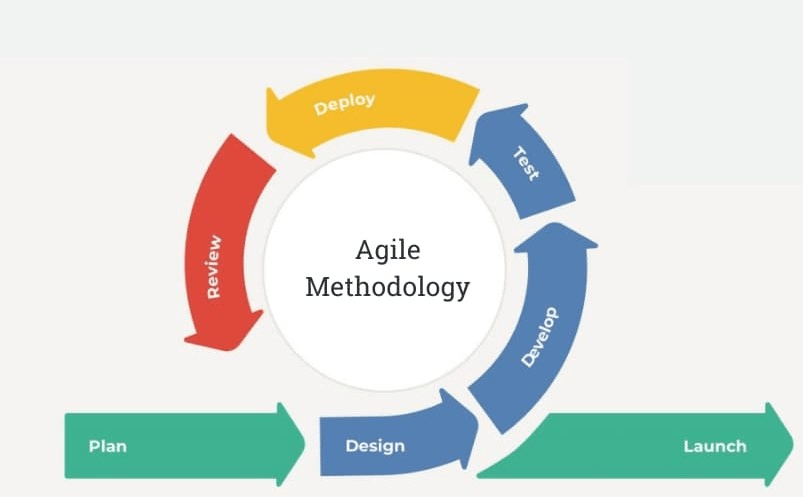
\includegraphics[width=0.85\linewidth,height=0.8\textheight,keepaspectratio]{Figures/agile_methodology.png}
\caption{Agile Methodology}
\label{fig:agilemethodology}
\end{figure}

\subsection{Justification of Proposing the Process Model}

The modules carry different levels of risk. Login, roles and exam set-up are well understood. Blocking Windows shortcut keys, the live dashboard, webcam analysis and running code in a Docker container were new to us. Waterfall would have forced us to fix all of these designs before we had built a prototype of any of them. With sprints we could try the risky parts early, integrate them step by step and adjust the plan. The sprint reviews at Weeks 16 and 32 also served as the FYP-I review and the final submission.

\subsection{Steps of Process Model}

The project runs over eight four-week sprints. Each sprint delivers modules that can be demonstrated. Table~\ref{tab:timeframe} in Chapter~\ref{chap:srs} gives the baseline schedule, and the text below it gives the progress at the FYP-I review. Every sprint goes through the following steps:
\begin{enumerate}[noitemsep]
\item \textbf{Product backlog:} FR1--FR12, grouped by module M1--M12 (Chapter~\ref{chap:srs}).
\item \textbf{Sprint planning:} a sprint goal and a sprint backlog in which each task has one WBS code and one owner.
\item \textbf{Development:} the module and its automated tests are written in the same sprint.
\item \textbf{Increment:} a task is done when its code and tests pass and its thesis section is updated.
\item \textbf{Sprint review:} the increment is demonstrated to the supervisor, who comments on it and on the backlog priorities.
\item \textbf{Schedule check:} if under 80\% of the story points are done, backlog items are moved or cut (Chapter~\ref{chap:spp}).
\item \textbf{Feedback:} review comments and accepted changes return to the product backlog.
\end{enumerate}
The baseline plan gives each sprint the following work:

\begin{itemize}[noitemsep]
\item \textbf{Sprint 1 (Weeks 1--4):} requirements, use cases, product backlog, architecture and scope approval.
\item \textbf{Sprint 2 (Weeks 5--8):} M1 and M7, with hardware-ID capture, device-bound student login, staff login and role-based access.
\item \textbf{Sprint 3 (Weeks 9--12):} M8 and M9, covering the exam wizard, question types, test cases, allowed applications and eligibility.
\item \textbf{Sprint 4 (Weeks 13--16):} M2, M3 and M4, covering the readiness check, practice exams, the student dashboard and the lockdown client.
\item \textbf{Sprint 5 (Weeks 17--20):} M5 and M10, with heartbeats, monitoring events and screenshots, and the live dashboard.
\item \textbf{Sprint 6 (Weeks 21--24):} M6 and M11, covering autosave, encrypted backup, test-case grading, TF-IDF theory scoring and the plagiarism matrix.
\item \textbf{Sprint 7 (Weeks 25--28):} M12, covering the hash-chained audit log, analytics, PDF reports, and Excel and evidence-ZIP exports.
\item \textbf{Sprint 8 (Weeks 29--32):} integration and system testing of all twelve modules, bug fixes, the final report and the demonstration.
\end{itemize}
